% Options for packages loaded elsewhere
\PassOptionsToPackage{unicode}{hyperref}
\PassOptionsToPackage{hyphens}{url}
\PassOptionsToPackage{dvipsnames,svgnames,x11names}{xcolor}
%
\documentclass[
]{article}

\usepackage{amsmath,amssymb}
\usepackage{iftex}
\ifPDFTeX
  \usepackage[T1]{fontenc}
  \usepackage[utf8]{inputenc}
  \usepackage{textcomp} % provide euro and other symbols
\else % if luatex or xetex
  \usepackage{unicode-math}
  \defaultfontfeatures{Scale=MatchLowercase}
  \defaultfontfeatures[\rmfamily]{Ligatures=TeX,Scale=1}
\fi
\usepackage{lmodern}
\ifPDFTeX\else  
    % xetex/luatex font selection
\fi
% Use upquote if available, for straight quotes in verbatim environments
\IfFileExists{upquote.sty}{\usepackage{upquote}}{}
\IfFileExists{microtype.sty}{% use microtype if available
  \usepackage[]{microtype}
  \UseMicrotypeSet[protrusion]{basicmath} % disable protrusion for tt fonts
}{}
\makeatletter
\@ifundefined{KOMAClassName}{% if non-KOMA class
  \IfFileExists{parskip.sty}{%
    \usepackage{parskip}
  }{% else
    \setlength{\parindent}{0pt}
    \setlength{\parskip}{6pt plus 2pt minus 1pt}}
}{% if KOMA class
  \KOMAoptions{parskip=half}}
\makeatother
\usepackage{xcolor}
\setlength{\emergencystretch}{3em} % prevent overfull lines
\setcounter{secnumdepth}{5}
% Make \paragraph and \subparagraph free-standing
\ifx\paragraph\undefined\else
  \let\oldparagraph\paragraph
  \renewcommand{\paragraph}[1]{\oldparagraph{#1}\mbox{}}
\fi
\ifx\subparagraph\undefined\else
  \let\oldsubparagraph\subparagraph
  \renewcommand{\subparagraph}[1]{\oldsubparagraph{#1}\mbox{}}
\fi


\providecommand{\tightlist}{%
  \setlength{\itemsep}{0pt}\setlength{\parskip}{0pt}}\usepackage{longtable,booktabs,array}
\usepackage{calc} % for calculating minipage widths
% Correct order of tables after \paragraph or \subparagraph
\usepackage{etoolbox}
\makeatletter
\patchcmd\longtable{\par}{\if@noskipsec\mbox{}\fi\par}{}{}
\makeatother
% Allow footnotes in longtable head/foot
\IfFileExists{footnotehyper.sty}{\usepackage{footnotehyper}}{\usepackage{footnote}}
\makesavenoteenv{longtable}
\usepackage{graphicx}
\makeatletter
\def\maxwidth{\ifdim\Gin@nat@width>\linewidth\linewidth\else\Gin@nat@width\fi}
\def\maxheight{\ifdim\Gin@nat@height>\textheight\textheight\else\Gin@nat@height\fi}
\makeatother
% Scale images if necessary, so that they will not overflow the page
% margins by default, and it is still possible to overwrite the defaults
% using explicit options in \includegraphics[width, height, ...]{}
\setkeys{Gin}{width=\maxwidth,height=\maxheight,keepaspectratio}
% Set default figure placement to htbp
\makeatletter
\def\fps@figure{htbp}
\makeatother
\newlength{\cslhangindent}
\setlength{\cslhangindent}{1.5em}
\newlength{\csllabelwidth}
\setlength{\csllabelwidth}{3em}
\newlength{\cslentryspacingunit} % times entry-spacing
\setlength{\cslentryspacingunit}{\parskip}
\newenvironment{CSLReferences}[2] % #1 hanging-ident, #2 entry spacing
 {% don't indent paragraphs
  \setlength{\parindent}{0pt}
  % turn on hanging indent if param 1 is 1
  \ifodd #1
  \let\oldpar\par
  \def\par{\hangindent=\cslhangindent\oldpar}
  \fi
  % set entry spacing
  \setlength{\parskip}{#2\cslentryspacingunit}
 }%
 {}
\usepackage{calc}
\newcommand{\CSLBlock}[1]{#1\hfill\break}
\newcommand{\CSLLeftMargin}[1]{\parbox[t]{\csllabelwidth}{#1}}
\newcommand{\CSLRightInline}[1]{\parbox[t]{\linewidth - \csllabelwidth}{#1}\break}
\newcommand{\CSLIndent}[1]{\hspace{\cslhangindent}#1}

\usepackage{booktabs}
\usepackage{longtable}
\usepackage{array}
\usepackage{multirow}
\usepackage{wrapfig}
\usepackage{float}
\usepackage{colortbl}
\usepackage{pdflscape}
\usepackage{tabu}
\usepackage{threeparttable}
\usepackage{threeparttablex}
\usepackage[normalem]{ulem}
\usepackage{makecell}
\usepackage{xcolor}
\usepackage[noblocks]{authblk}
\renewcommand*{\Authsep}{, }
\renewcommand*{\Authand}{, }
\renewcommand*{\Authands}{, }
\renewcommand\Affilfont{\small}
\makeatletter
\makeatother
\makeatletter
\makeatother
\makeatletter
\@ifpackageloaded{caption}{}{\usepackage{caption}}
\AtBeginDocument{%
\ifdefined\contentsname
  \renewcommand*\contentsname{Table of contents}
\else
  \newcommand\contentsname{Table of contents}
\fi
\ifdefined\listfigurename
  \renewcommand*\listfigurename{List of Figures}
\else
  \newcommand\listfigurename{List of Figures}
\fi
\ifdefined\listtablename
  \renewcommand*\listtablename{List of Tables}
\else
  \newcommand\listtablename{List of Tables}
\fi
\ifdefined\figurename
  \renewcommand*\figurename{Figure}
\else
  \newcommand\figurename{Figure}
\fi
\ifdefined\tablename
  \renewcommand*\tablename{Table}
\else
  \newcommand\tablename{Table}
\fi
}
\@ifpackageloaded{float}{}{\usepackage{float}}
\floatstyle{ruled}
\@ifundefined{c@chapter}{\newfloat{codelisting}{h}{lop}}{\newfloat{codelisting}{h}{lop}[chapter]}
\floatname{codelisting}{Listing}
\newcommand*\listoflistings{\listof{codelisting}{List of Listings}}
\makeatother
\makeatletter
\@ifpackageloaded{caption}{}{\usepackage{caption}}
\@ifpackageloaded{subcaption}{}{\usepackage{subcaption}}
\makeatother
\makeatletter
\@ifpackageloaded{tcolorbox}{}{\usepackage[skins,breakable]{tcolorbox}}
\makeatother
\makeatletter
\@ifundefined{shadecolor}{\definecolor{shadecolor}{rgb}{.97, .97, .97}}
\makeatother
\makeatletter
\makeatother
\makeatletter
\makeatother
\ifLuaTeX
  \usepackage{selnolig}  % disable illegal ligatures
\fi
\IfFileExists{bookmark.sty}{\usepackage{bookmark}}{\usepackage{hyperref}}
\IfFileExists{xurl.sty}{\usepackage{xurl}}{} % add URL line breaks if available
\urlstyle{same} % disable monospaced font for URLs
\hypersetup{
  pdftitle={Title of Report},
  pdfauthor={Libby Brill; Sophia Freije; Jett Palmer; Alea Seifert},
  colorlinks=true,
  linkcolor={blue},
  filecolor={Maroon},
  citecolor={Blue},
  urlcolor={Blue},
  pdfcreator={LaTeX via pandoc}}

\title{Title of Report}


\author[1]{Libby Brill}
\author[1]{Sophia Freije}
\author[1]{Jett Palmer}
\author[1]{Alea Seifert}

\affil[1]{Department of Statistics, Cal Poly - SLO}


\date{May 31, 2024}
\begin{document}
\maketitle
\begin{abstract}
Your abstract goes here (max \textasciitilde250 words).
\end{abstract}
\ifdefined\Shaded\renewenvironment{Shaded}{\begin{tcolorbox}[borderline west={3pt}{0pt}{shadecolor}, sharp corners, breakable, boxrule=0pt, enhanced, frame hidden, interior hidden]}{\end{tcolorbox}}\fi

\hypertarget{abstract}{%
\section{Abstract}\label{abstract}}

The London Fire Brigade (LBF) is a firefighting and rescue organization
that receives various calls regarding animal rescues from London
citizens. Within the LBF recorded rescues, spanning from 2009 to 2020,
there was a noticeable difference observed in the number of wild animals
(n = 4668) and pet calls (n = 1898). We analyzed data using statistical
software to understand the impact of time on the frequency of animal
rescues based on animal type. Through a two-proportion z-test, we found
a discernible difference in the percentage of night-time incidents
comparing pets and wild animals. With a broad span of services conducted
by the LBF, information regarding the frequency of pet rescues during
the night-time is helpful when allocating resources and scheduling
staff. This allows the LBF to be better equipped to handle pet rescue
incidents most efficiently during the night shift.

\hypertarget{intro}{%
\section{Introduction}\label{intro}}

Every year, hundreds of animals across London find themselves in need of
rescue - ranging from cats trapped in a tree to ducklings fallen into
storm drains. But who does one call when they find an animal in
distress? Members of the public are encouraged to first call the Royal
Society for the Prevention of Cruelty to Animals (RSPCA) when they
encounter an animal in trouble. However, in situations where specialized
equipment is required or when the caller forgoes reporting to RSPCA
first, the London Fire Brigade (LFB) is summoned.

The London Fire Brigade has spent over 2.5 million pounds
(\textasciitilde3.2 million US dollars) on animal rescues (Boyle, 2023).
Considering that the fire brigade's primary objective is safeguarding
the people of London and protecting their property from fire, not animal
safety, this is quite a substantial sum. While we believe the fire
brigade should continue promoting animal welfare, we aim to reduce their
burden and increase readiness by examining the most difficult time for
animal rescue: night-time. Animal rescues made during the night are more
difficult because of the lower visibility and need for adherence to
quiet hours as residents sleep.

The animal rescue calls can be divided into two main categories, pets
and wild animals. There were more calls made for pets compared to wild
animals. Taking these unequal counts into consideration, we aim to
discover if there is a discernible difference in the proportion of
night-time rescues between pets and wild animals.

According to Tuan et al. (2015), it is said to xxx. Supported by this we
found xyz (Wiwanitkit 2010).

\hypertarget{data-and-methods}{%
\section{Data and Methods}\label{data-and-methods}}

\hypertarget{data-description}{%
\subsection{Data Description}\label{data-description}}

Each observation represents one concerned citizen's call to the London
Fire Brigade about an animal in distress. The only qualification for a
phone call to be recorded was it had to concern an animal rescue within
one of London's 32 boroughs - any incident involving or resulting in
animal injury or death was not recorded. After each call, the time that
the call was made (including the date and hour of the call) was
documented. Then, after the firefighters performed the rescue,
information pertaining to the incident's exact location within London,
type of animal, type of rescue performed, and cost were recorded. For
the purpose of answering if there is a significant difference in
proportions between pets and wild animals night-time rescues, we will
only examine the time of day, year, and type of animal.

The data were collected from January 2009 were updated monthly to the
London Data Store {[}needs citation here{]} until May 2021. Considering
the 2021 data does not cover the entire year, we only examined calls
made up to the end of 2020. Over this twelve year period, 7,225 animal
rescue calls were made.

\hypertarget{statistical-analysis}{%
\subsection{Statistical Analysis}\label{statistical-analysis}}

In order to assess variance between different groups of animals, we
needed to define some species as ``wild'' and others as ``pets.'' While
this process was ultimately subjective, we consulted online sources to
guide the decision (Messmer 2020). We labeled cats, dogs, and rabbits as
pets, and considered birds, foxes, and deer as wild animals. Similarly,
we decided that incidents occurring from 6:00 pm to 5:59 am would be
considered night-time rescues whereas the remaining times are day-time
incidents

There is a sufficient number of night-time and day-time rescues for both
groups, and we assume that observations are independent from each other,
with one animal rescue not influencing the next. Thus, we conducted a
two-proportion z-test to investigate whether the proportion of
night-time rescues is different between pets and wild animals.

The analyses were conducted in (\textbf{Manual?}) using INSERT PACKAGE
CITATIONS.

\hypertarget{results}{%
\section{Results}\label{results}}

As seen in Table 1, the proportion of night-time incidents for pets and
wild animals are 35\% and 30\%, respectively. We should note that a much
larger number of pet incidents occurred, compared to wild animals, when
investigating sample sizes.

\hypertarget{tbl-night-summary}{}
\begin{table}
\caption{\label{tbl-night-summary}The table depicts the percentage of night-time animal rescues by the
London Fire Brigade from 2009 to 2020 of pets and wild animals. The
table also includes the total number of calls for each group. }\tabularnewline

\centering
\begin{tabular}[t]{lcc}
\toprule
Animal Type & \% of Rescues Occuring at Night & Total Number of Animals\\
\midrule
Pets & 35.0\% & 4668\\
Wild Animals & 30.0\% & 1898\\
\bottomrule
\end{tabular}
\end{table}

Figure 1 further illustrates these results while also indicating trends
over time. Notably, there were several years in which the year-over-year
trend was different between the two groups. For example, from 2017 to
2019, the proportion of night-time incidents for wild animals dipped,
contrasting the pet proportions that showed continuous increases.

\begin{figure}[H]

{\centering 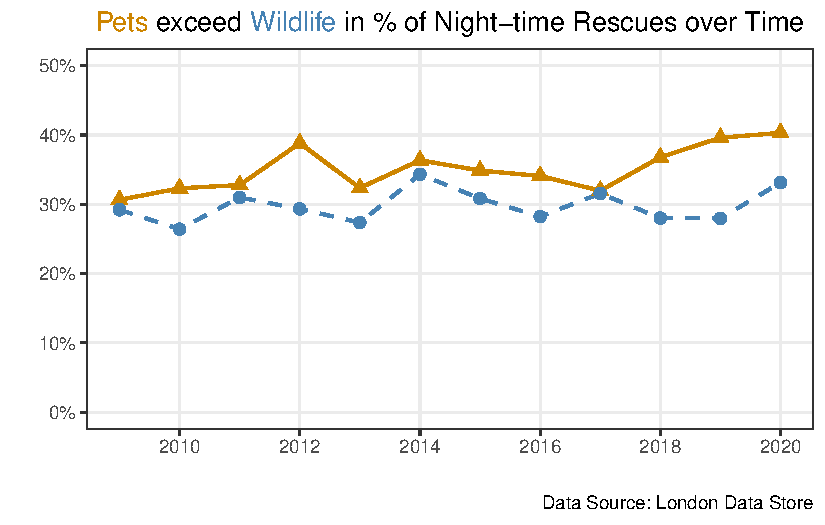
\includegraphics{Final_Report_files/figure-pdf/fig-night-animal-1.pdf}

}

\caption{\label{fig-night-animal}The figure represents the percentage of
night-time animal rescues by the London Fire Brigade from 2009 to 2020.
Grouped by pets (cat, dog, rabbit) and wild animals (bird, fox, deer),
the plot reveals that the percent of pet night rescues is larger than
wildlife night rescues across all years.}

\end{figure}

Figure 2 indicates greater variability within the wild animal group
which may be a product of the lower comparative sample size.
Importantly, we note that the margin of error does not overlap between
the two groups, providing visual evidence of a significant difference in
proportions of night-time incidents. Consequently, after running the
two-proportion z-test, we found a discernible difference in the
proportion of night-time incidents between pets and wild animals (X2 =
14.991; df = 1; p-value \textless{} 0.0001).

INSERT CONFIDENCE INTERVAL PLOT

\hypertarget{discussion}{%
\section{Discussion}\label{discussion}}

Based on our findings, we can draw a few observations about LFB animal
rescues. Namely, we found there is a significant difference between the
proportion of pet rescues and wild animal rescues during the night-time
hour. This means that pets proportionally get into trouble at night more
often than wild animals. To fully understand if this difference has any
practical significance we recommend consulting with licensed wildlife
rehabbers or other professional animal caretakers. These professionals
might better understand how various external factors other than time of
day influence animal incidents. For instance, time of year might be a
factor to include in future studies as spring months that fall under
``baby season'' could potentially have more incidents.

It is important to note that we can not generalize our findings to all
types of pets. Domesticated animals including horses, goats, and guinea
pigs were not included. The subjective categorization of animals into
pet and wild groups is also a limitation of our findings. The data do
not provide information to check the accuracy of our categorization and,
thus, it is possible that some animals are incorrectly represented as in
our analysis. For instance, domestic bird incidents may be tabulated in
our results under wild animal incidents.

Table~\ref{tbl-night-summary} Figure~\ref{fig-night-animal}

\hypertarget{conclusion}{%
\section{Conclusion}\label{conclusion}}

Our analysis of the London Fire Brigade's data on animal rescues
provided valuable insights into the patterns of night-time incidents
involving pets and wild animals. Our findings indicate that pets
(defined as dogs, cats, and rabbits) have a significantly higher rate of
night-time rescues compared to wild animals (foxes, deer, and birds).
This suggests a need for increased public awareness regarding pet
safety. Ensuring that pets are in secure locations overnight can
potentially reduce the number of night-time rescues, enhancing both pet
safety and the efficiency of rescue operations.

While our analysis specifically focused on the proportion of night-time
rescues, it can be noted that the majority of incidents for both pets
and wild animals occurred during the day, with night-time rescues making
up less than 36\% of the total incidents for both groups. This
information is important for the LFB, as it highlights the periods when
more resources and personnel are likely needed to effectively respond to
animal rescue calls.

Future research might delve deeper into the specifics of these rescue
incidents, such as the types of rescues (e.g., rescues from a height,
water rescues, rescues below ground) that are most common for both pets
and wild animals. Such analyses could further enhance the LFB's
preparedness and response strategies, ensuring that they are
well-equipped to handle the challenges presented by different rescue
scenarios.

It is also important to acknowledge the limitations of our study. Given
that our data disregards any animal injuries or death, our results can
not be applied to calls where animals are life threatening predicaments.
Additionally, our analysis encompasses the entire population of reported
rescues by the LFB from 2009 to 2021, thus there is no larger population
to which we can generalize our results. Nonetheless, our results provide
a foundational understanding of animal rescue patterns in London,
offering practical insights that can inform both public safety measures
and the operational strategies of the LFB.

\hypertarget{references}{%
\section*{References}\label{references}}
\addcontentsline{toc}{section}{References}

\hypertarget{refs}{}
\begin{CSLReferences}{1}{0}
\leavevmode\vadjust pre{\hypertarget{ref-tuan2015}{}}%
Tuan, Nguyen Minh, Ho Thi Nhan, Nguyen Van Vinh Chau, Nguyen Thanh Hung,
Ha Manh Tuan, Ta Van Tram, Nguyen Le Da Ha, et al. 2015. {``Sensitivity
and Specificity of a Novel Classifier for the Early Diagnosis of
Dengue.''} Edited by Scott B Halstead. \emph{PLOS Neglected Tropical
Diseases} 9 (4): e0003638.
\url{https://doi.org/10.1371/journal.pntd.0003638}.

\leavevmode\vadjust pre{\hypertarget{ref-wiwanitkit2010dengue}{}}%
Wiwanitkit, Viroj. 2010. {``Dengue Fever: Diagnosis and Treatment.''}
\emph{Expert Review of Anti-Infective Therapy} 8 (7): 841--45.

\end{CSLReferences}



\end{document}
